\appendix

\subsection{\acrlong{ppm}}

\begin{figure}[H]
\centering
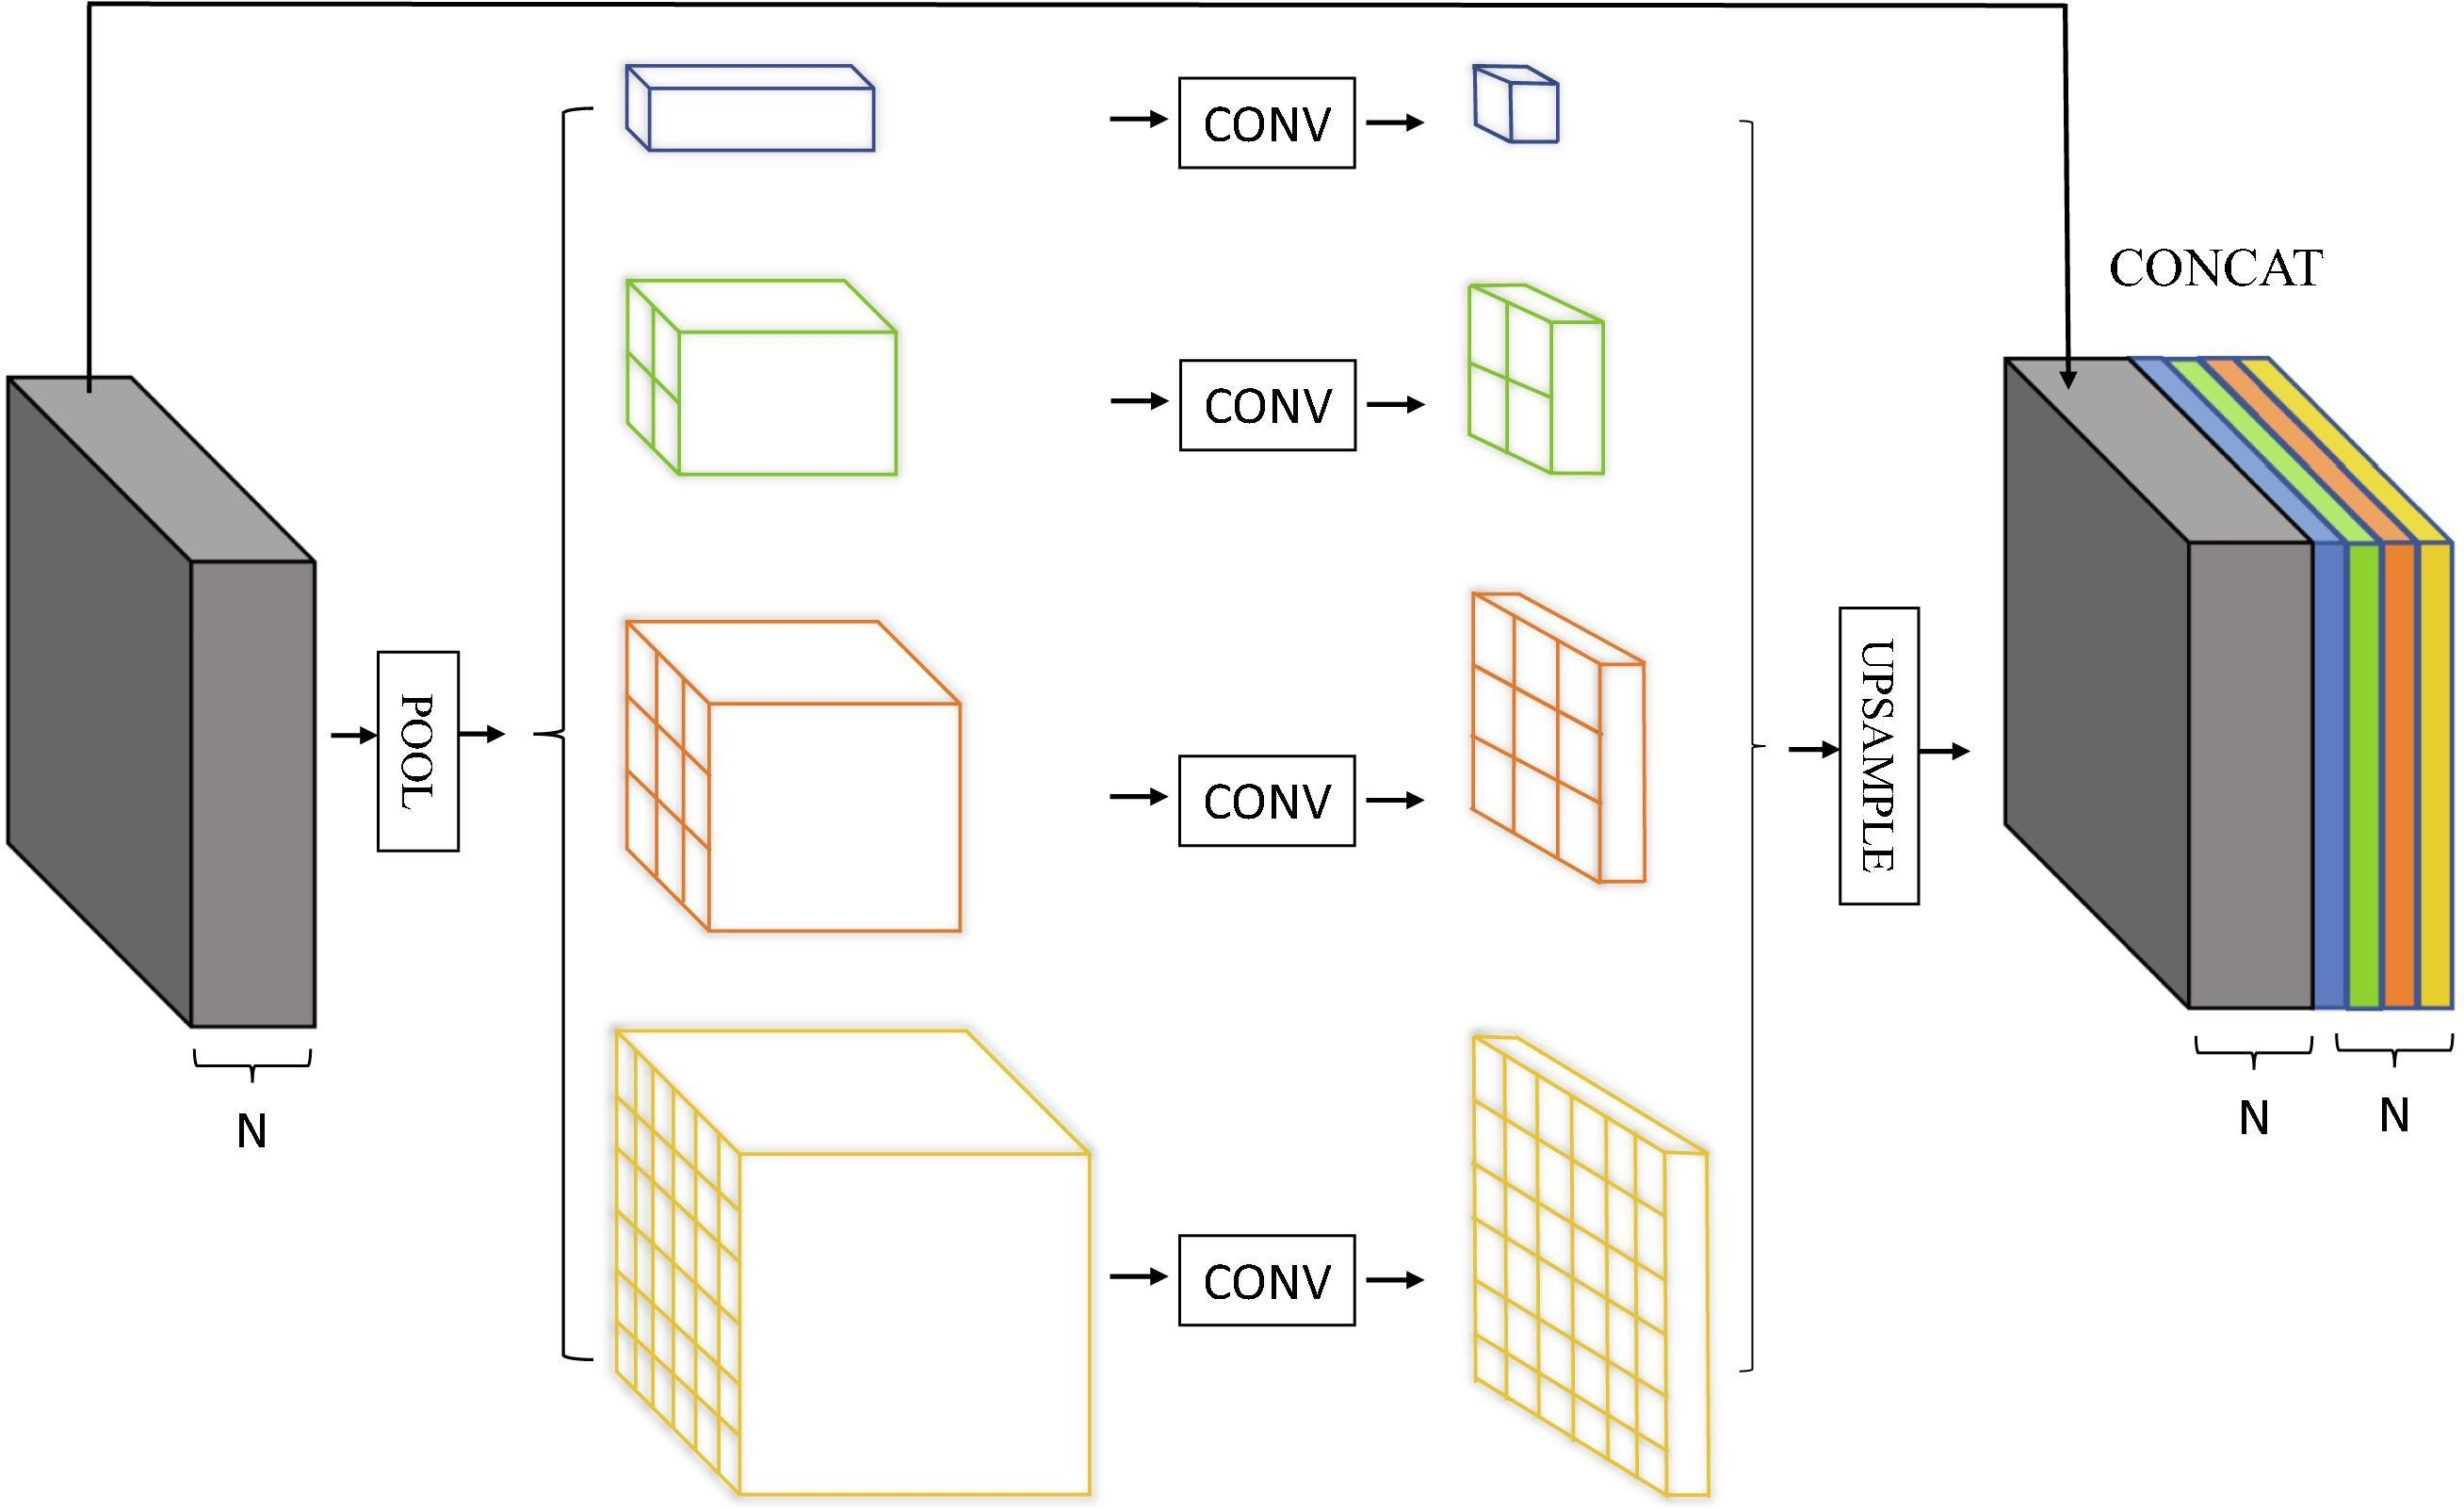
\includegraphics[width=1.0\linewidth]{images/pyrmid-pooling.jpg}
\caption{\acrlong{ppm} used in \acrshort{gcdcnn} \cite{gcdcnn}}
\label{fig:ppm}
\end{figure}

\subsection{Augmentation parameters}
In total we experimented with over twenty different augmentations. A key result of these experiments is, that if \acrfull{ssr} is not applied the model overfits and achieves a training accuracy of over 99\%. For brevity, we here only list the explanation of the top three augmentations.
\begin{itemize}
    \item \acrfull{ssr}: Randomly shift, scale and rotate the image. We uniformly draw a shift value in [-0.0625, 0.0625], a scale value in [-0.1, 0.1] and a rotation value in [-45, 45] degrees. % We use BORDER_REFLECT_101 which mirrors the border...
    % \item \acrfull{cs}: The three channels RGB are shuffled randomly.
    \item \acrfull{rc}: Change the contrast with a random factor in the range  [-0.2, 0.2]
    \item \acrfull{gn}: We apply Gaussian noise with a mean of 0 and a variance limit of [10.0, 50.0]. % not clear what the variance parameter of the Gaussian is set to; maybe a uniformly drawn value from the limit interval?
\end{itemize}

\subsection{Results of architecture alterations}

\subsubsection{U-Net}

In the following we list the explanations of the different \acrshort{unet} architecture tunings of which the results can be found in table \ref{tab:unet_alt}.
\begin{itemize}
    \item Dilation: Dilations with factors 3 and 18 were applied to all filters
    \item Filtersize: Filtersize was increased to 5 instead of 3
    \item PoolKernel: The Max Pooling kernel was increased to size 4 instead of 2
    \item Dilation and LR-Change: Dilation with factor 3 with a initial learning rate of $10^{-4}$ instead of $10^{-3}$
\end{itemize}

\begin{table}[h!]
    \centering
    \begin{tabular}{l|p{0.15\linewidth}|p{0.15\linewidth}|p{0.15\linewidth}}
         method & Validation Accuracy  & Public Score & Best Epoch  \\
         \hline
         Baseline U-Net & \textbf{97.185} & 92.352 & 124\\
         Dilation (3) & 96.817 & 91.942 & 34\\
         Dilation (18) & 96.280 & 90.941 & 86\\
         Filtersize (5) & 97.123 & 92.793 & 105\\
         PoolKernel (4) & 97.169 & \textbf{92.809} & 149\\
         Dilation (3) lr=$10^{-4}$ & 97.110 & 92.203 & 70\\
    \end{tabular}
    \caption{Results of U-Net Architecture Alterations}
    \label{tab:unet_alt}
\end{table}

\subsubsection{GC-DCNN}

%The results in table \ref{tab:gcdcnn_tuning} show that different architecture modifications do not change the validation accuracy by a lot. Considering that the experiments dataset consists of multiple datasets (ETH, GMaps-public) with different ground truth labeling technique, we reason that the validation score is close to the optimal.
Results of architecture variations of the \acrshort{gcdcnn} can be seen in Table \ref{tab:gcdcnn_tuning}. As our final model we choose the model ASPP + Attention + Deep, since it achieved the best validation score as well as a high public score.

\begin{table}[h!]
    \centering
    \begin{tabular}{l|p{0.15\linewidth}|p{0.15\linewidth}|p{0.15\linewidth}}
         Method & Validation Accuracy & Public Score & Best Epoch  \\ \hline
         - & 97.270 & 92.242 & 71 \\ % 20210626-222336-0004_gcdcnn_exp_augmentation
         Attention & 97.279 & 92.246 & 60 \\ % 20210626-093027-gcdcnn_exp_attention
         ASPP & 97.3 & \textbf{92.549} & 97 \\ % 20210626-093027-gcdcnn_exp_aspp_avg_pool
         ASPP + Attention & 97.145 & 92.201 & 51 \\ % 20210626-111758-gcdcnn_exp_aspp_avg_pool_attention
         Deep & 97.272 & 92.195 & 178 \\ % 20210626-092358-gcdcnn_exp_deep
         ASPP + Deep & 97.301 & \textbf{92.468} & 105 \\ % 20210625-200334-gcdcnn_exp_deep_aspp_avg_pool
         Attention + Deep & 97.235  & 92.049 & 102  \\ % 20210625-215203-gcdcnn_exp_deep_attention
         ASPP + Attention + Deep & \textbf{97.319} & \textbf{92.430} & 132 \\ % 20210625-205535-gcdcnn_exp_deep_aspp_avg_pool_attention
    \end{tabular}
    \caption{Results of \acrshort{gcdcnn} Architecture Alterations}
    \label{tab:gcdcnn_tuning}
\end{table}


%  \begin{table}[h!]
%      \centering
%      \begin{tabular}{l|l|p{0.10\linewidth}|p{0.10\linewidth}|p{0.05\linewidth}}
%           Model & Validation Acc & Public Score & Dilation\\ \hline
%     UNET &  0.97563 & - & -\\\hline % 20210704-202654-unet_exp_template
%     Retrain UNET &  0.98141 & - & 1\\ % 20210706-174459-unet_exp_template
%     Retrain UNET  & 0.98146  & - & 5\\ % 20210706-175301-unet_exp_dilation_5
%     Retrain UNET &  0.98148 & - & 7\\ %20210706-175332-unet_exp_dilation_7
%     \hline
%     Retrain UNET-PCONV & 0.98165 & - & 1\\ %20210707-213909-unet_pconv_exp_template
%     Retrain UNET-PCONV & 0.98142 & - & 3\\ %20210707-215537-unet_pconv_exp_dilation_3
%     Retrain UNET-PCONV & 0.98149 & - & 5\\ %20210707-215538-unet_pconv_exp_dilation_5
%     Retrain UNET-PCONV & 0.98148 & - & 7\\ %20210707-215539-unet_pconv_exp_dilation_7
%      \end{tabular}
%      \caption{Results of retraining on binary images}
%      \label{tab:postprocessing}
%  \end{table}
 
\subsection{Postprocessing results}
 
\begin{table}[H]
    \centering
    \begin{tabular}{l|p{0.15\linewidth}|p{0.15\linewidth}|p{0.10\linewidth}}
        Model & Validation Accuracy & Public Score & Dilation\\ \hline
        \acrshort{unet}-plus &  96.150 & 92.835 & -\\\hline % 
        Retrain \acrshort{unet} & \textbf{97.433} & 92.964 & 1\\ % 
        Retrain \acrshort{unet}  &  97.449 & \textbf{93.034} & 5\\ % 
%        Retrain \acrshort{unet} &  97.410 & 92.961 & 7\\ %
        \hline
        Retrain \acrshort{unet}-PCONV & 97.439 & 92.987 & 1\\ %
        Retrain \acrshort{unet}-PCONV & 97.450 & 93.001 & 3\\ %
        Retrain \acrshort{unet}-PCONV & 97.422 & 93.028 & 5\\ %
%        Retrain \acrshort{unet}-PCONV & 97.429 & 92.999 & 7\\ %
    \end{tabular}
    \caption{Results of postprocessing binary retraining using \acrshort{unet} on \acrshort{unet}-plus predictions}
    \label{tab:postprocessingunet}
\end{table}
 
 
\begin{table}[H]
    \centering
    \begin{tabular}{l|p{0.15\linewidth}|p{0.15\linewidth}|p{0.10\linewidth}}
        Model & Validation Accuracy & Public Score & Dilation\\ \hline
        GCDCNN-plus&  96.28 & 92.99 & -\\\hline % 
        Retrain \acrshort{unet} &  97.484 & 93.032 & 1\\ % 
        Retrain \acrshort{unet}  & 97.480  & \textbf{93.065} & 5\\ % 
%        Retrain \acrshort{unet} &  97.493 & 93.041 & 7\\ %
        \hline
        Retrain \acrshort{unet}-PCONV & 97.490 & 93.041 & 1\\ %
        Retrain \acrshort{unet}-PCONV &  97.547 & 93.038 & 3\\ %
        Retrain \acrshort{unet}-PCONV & \textbf{97.485} & 93.029 & 5\\ %
%        Retrain \acrshort{unet}-PCONV &  97.493 & 93.029 & 7\\ %
    \end{tabular}
    \caption{Results of postprocessing binary retraining using \acrshort{unet} on \acrshort{gcdcnn}-plus predictions}
    \label{tab:postprocessinggcdcnn}
\end{table}



